%---------------------------------------------------------
%	5. MODEL INTERPRETABILITY
%	SHAP / feature importance do not fit an image-to-image model; component ablation plays that role.
%---------------------------------------------------------
\begin{frame}
    \frametitle{Model Interpretability (1/2): Which Components Matter?}
    \framesubtitle{Component importance = PSNR lost when a part is removed or replaced (paper ablations)}

    \begin{center}
        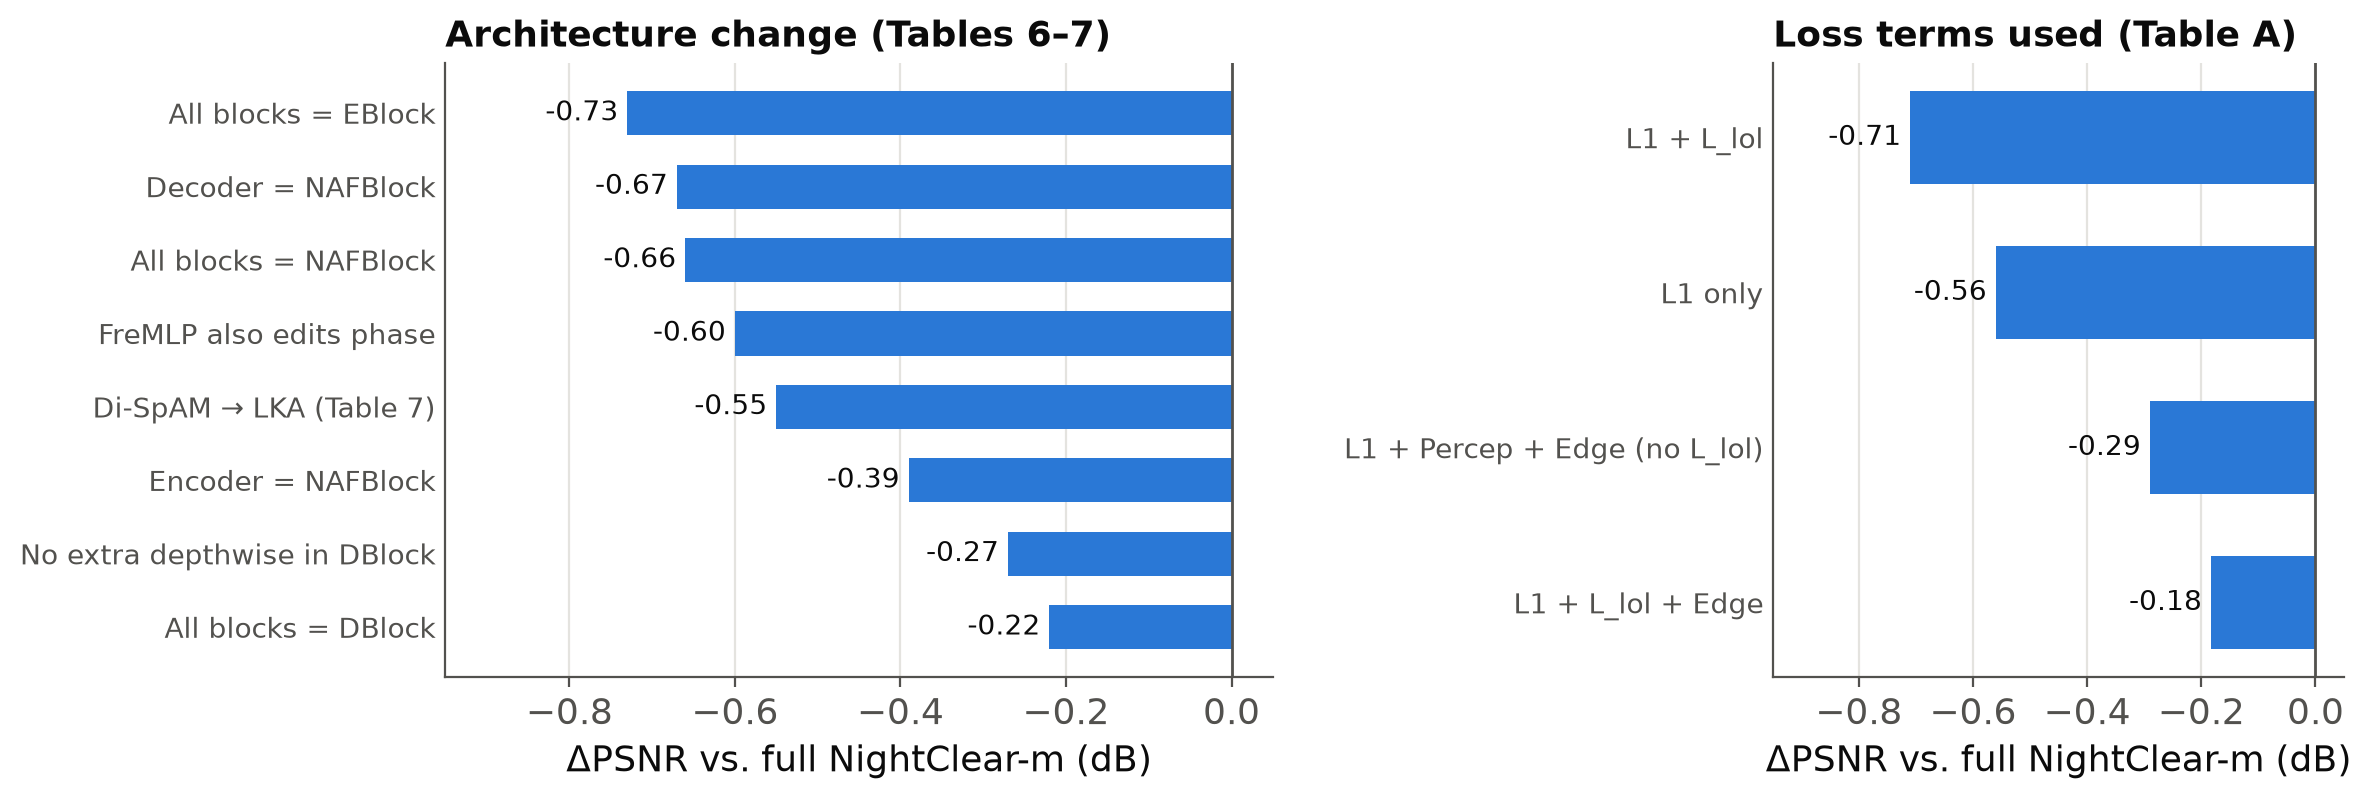
\includegraphics[width=\textwidth, height=0.47\textheight, keepaspectratio]{results/ablation.png}
    \end{center}
    \footnotesize
    \begin{itemize}
        \item Using the \textbf{same block everywhere} costs up to 0.73\,dB: the encoder (illumination) and the decoder (deblurring) need different designs.
        \item The low-res supervision $\mathcal{L}_{\text{low-res}}$ only helps together with the perceptual and edge losses (all four terms give the best PSNR).
    \end{itemize}
    {\tiny Table 6 and A: 256\,px training crops, full model 26.90\,dB; Table 7: full model 27.00\,dB.}
\end{frame}

\begin{frame}
    \frametitle{Model Interpretability (2/2): Why the Fourier Amplitude?}
    \framesubtitle{Our experiment on the 100 LOLv2-real test pairs: swap the FFT amplitude, keep the phase}

    \begin{center}
        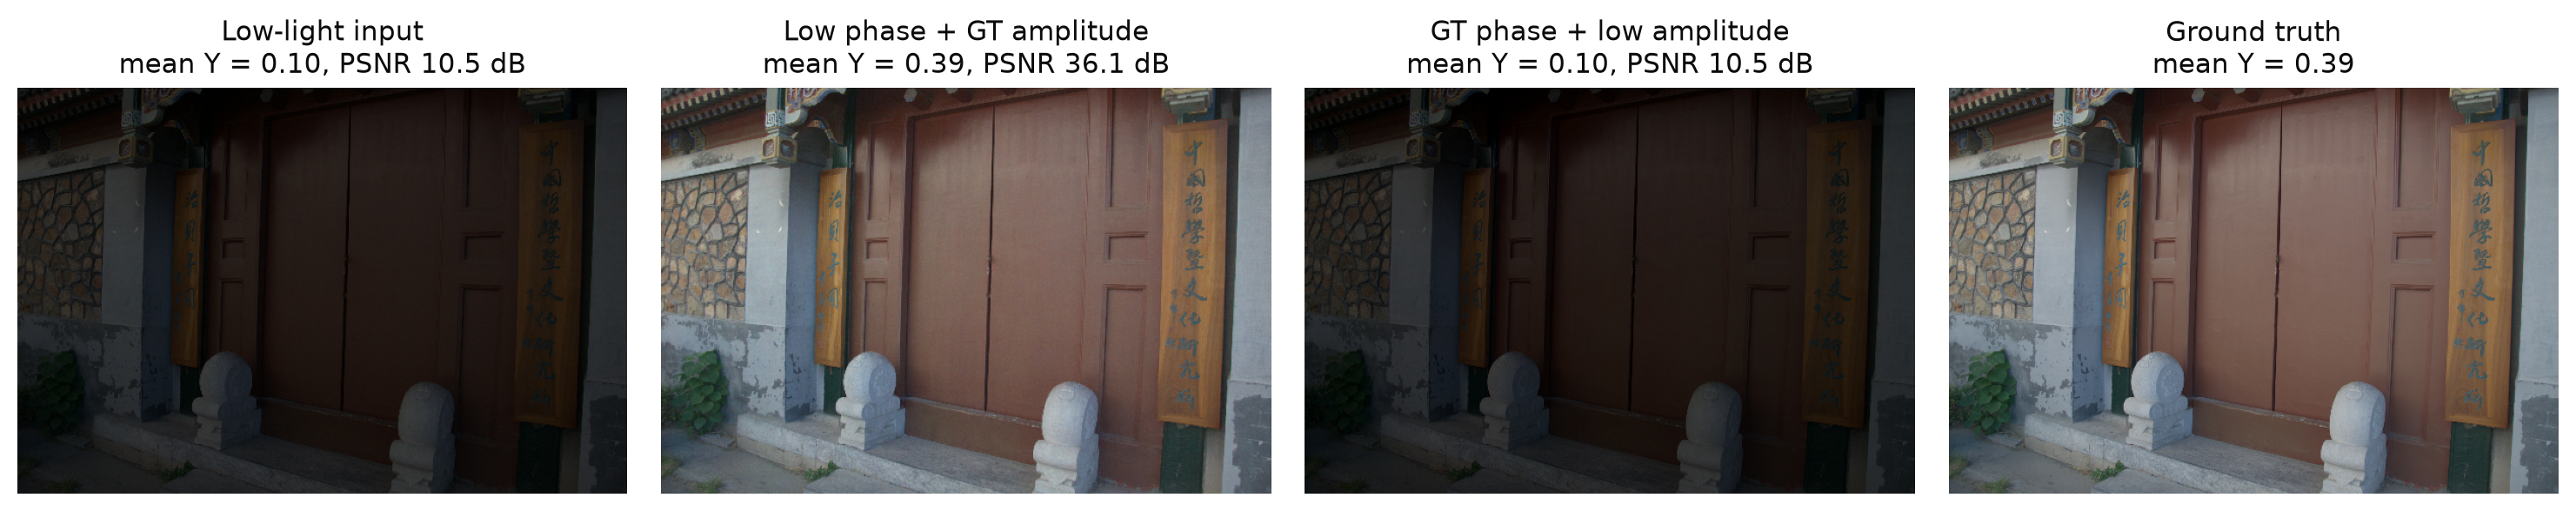
\includegraphics[width=\textwidth, height=0.36\textheight, keepaspectratio]{results/amplitude_swap.png}
    \end{center}
    \begin{columns}[t]
        \begin{column}{0.55\textwidth}
            \footnotesize
            \begin{itemize}
                \item Low-light \textbf{phase} + GT \textbf{amplitude} $\approx$ the GT image: mean PSNR \textbf{9.72 $\rightarrow$ 29.07\,dB} over 100 pairs.
                \item GT phase + low amplitude stays dark: brightness lives in the amplitude, structure in the phase.
            \end{itemize}
        \end{column}
        \begin{column}{0.43\textwidth}
            \footnotesize
            $\Rightarrow$ This explains the design: \textbf{FreMLP} edits only the amplitude, and letting it change the phase too \textbf{lowers PSNR by 0.60\,dB} (Table 6).
        \end{column}
    \end{columns}
\end{frame}
